\PassOptionsToPackage{unicode=true}{hyperref} % options for packages loaded elsewhere
\PassOptionsToPackage{hyphens}{url}
%
\documentclass[
]{article}
\usepackage{lmodern}
\usepackage{amssymb,amsmath}
\usepackage{ifxetex,ifluatex}
\ifnum 0\ifxetex 1\fi\ifluatex 1\fi=0 % if pdftex
  \usepackage[T1]{fontenc}
  \usepackage[utf8]{inputenc}
  \usepackage{textcomp} % provides euro and other symbols
\else % if luatex or xelatex
  \usepackage{unicode-math}
  \defaultfontfeatures{Scale=MatchLowercase}
  \defaultfontfeatures[\rmfamily]{Ligatures=TeX,Scale=1}
\fi
% use upquote if available, for straight quotes in verbatim environments
\IfFileExists{upquote.sty}{\usepackage{upquote}}{}
\IfFileExists{microtype.sty}{% use microtype if available
  \usepackage[]{microtype}
  \UseMicrotypeSet[protrusion]{basicmath} % disable protrusion for tt fonts
}{}
\makeatletter
\@ifundefined{KOMAClassName}{% if non-KOMA class
  \IfFileExists{parskip.sty}{%
    \usepackage{parskip}
  }{% else
    \setlength{\parindent}{0pt}
    \setlength{\parskip}{6pt plus 2pt minus 1pt}}
}{% if KOMA class
  \KOMAoptions{parskip=half}}
\makeatother
\usepackage{xcolor}
\IfFileExists{xurl.sty}{\usepackage{xurl}}{} % add URL line breaks if available
\IfFileExists{bookmark.sty}{\usepackage{bookmark}}{\usepackage{hyperref}}
\hypersetup{
  pdftitle={Liu-West Filter for a building Grey-box model},
  pdfauthor={Sang woo Ham},
  pdfborder={0 0 0},
  breaklinks=true}
\urlstyle{same}  % don't use monospace font for urls
\usepackage[margin=1in]{geometry}
\usepackage{color}
\usepackage{fancyvrb}
\newcommand{\VerbBar}{|}
\newcommand{\VERB}{\Verb[commandchars=\\\{\}]}
\DefineVerbatimEnvironment{Highlighting}{Verbatim}{commandchars=\\\{\}}
% Add ',fontsize=\small' for more characters per line
\usepackage{framed}
\definecolor{shadecolor}{RGB}{248,248,248}
\newenvironment{Shaded}{\begin{snugshade}}{\end{snugshade}}
\newcommand{\AlertTok}[1]{\textcolor[rgb]{0.94,0.16,0.16}{#1}}
\newcommand{\AnnotationTok}[1]{\textcolor[rgb]{0.56,0.35,0.01}{\textbf{\textit{#1}}}}
\newcommand{\AttributeTok}[1]{\textcolor[rgb]{0.77,0.63,0.00}{#1}}
\newcommand{\BaseNTok}[1]{\textcolor[rgb]{0.00,0.00,0.81}{#1}}
\newcommand{\BuiltInTok}[1]{#1}
\newcommand{\CharTok}[1]{\textcolor[rgb]{0.31,0.60,0.02}{#1}}
\newcommand{\CommentTok}[1]{\textcolor[rgb]{0.56,0.35,0.01}{\textit{#1}}}
\newcommand{\CommentVarTok}[1]{\textcolor[rgb]{0.56,0.35,0.01}{\textbf{\textit{#1}}}}
\newcommand{\ConstantTok}[1]{\textcolor[rgb]{0.00,0.00,0.00}{#1}}
\newcommand{\ControlFlowTok}[1]{\textcolor[rgb]{0.13,0.29,0.53}{\textbf{#1}}}
\newcommand{\DataTypeTok}[1]{\textcolor[rgb]{0.13,0.29,0.53}{#1}}
\newcommand{\DecValTok}[1]{\textcolor[rgb]{0.00,0.00,0.81}{#1}}
\newcommand{\DocumentationTok}[1]{\textcolor[rgb]{0.56,0.35,0.01}{\textbf{\textit{#1}}}}
\newcommand{\ErrorTok}[1]{\textcolor[rgb]{0.64,0.00,0.00}{\textbf{#1}}}
\newcommand{\ExtensionTok}[1]{#1}
\newcommand{\FloatTok}[1]{\textcolor[rgb]{0.00,0.00,0.81}{#1}}
\newcommand{\FunctionTok}[1]{\textcolor[rgb]{0.00,0.00,0.00}{#1}}
\newcommand{\ImportTok}[1]{#1}
\newcommand{\InformationTok}[1]{\textcolor[rgb]{0.56,0.35,0.01}{\textbf{\textit{#1}}}}
\newcommand{\KeywordTok}[1]{\textcolor[rgb]{0.13,0.29,0.53}{\textbf{#1}}}
\newcommand{\NormalTok}[1]{#1}
\newcommand{\OperatorTok}[1]{\textcolor[rgb]{0.81,0.36,0.00}{\textbf{#1}}}
\newcommand{\OtherTok}[1]{\textcolor[rgb]{0.56,0.35,0.01}{#1}}
\newcommand{\PreprocessorTok}[1]{\textcolor[rgb]{0.56,0.35,0.01}{\textit{#1}}}
\newcommand{\RegionMarkerTok}[1]{#1}
\newcommand{\SpecialCharTok}[1]{\textcolor[rgb]{0.00,0.00,0.00}{#1}}
\newcommand{\SpecialStringTok}[1]{\textcolor[rgb]{0.31,0.60,0.02}{#1}}
\newcommand{\StringTok}[1]{\textcolor[rgb]{0.31,0.60,0.02}{#1}}
\newcommand{\VariableTok}[1]{\textcolor[rgb]{0.00,0.00,0.00}{#1}}
\newcommand{\VerbatimStringTok}[1]{\textcolor[rgb]{0.31,0.60,0.02}{#1}}
\newcommand{\WarningTok}[1]{\textcolor[rgb]{0.56,0.35,0.01}{\textbf{\textit{#1}}}}
\usepackage{longtable,booktabs}
% Allow footnotes in longtable head/foot
\IfFileExists{footnotehyper.sty}{\usepackage{footnotehyper}}{\usepackage{footnote}}
\makesavenoteenv{longtable}
\usepackage{graphicx,grffile}
\makeatletter
\def\maxwidth{\ifdim\Gin@nat@width>\linewidth\linewidth\else\Gin@nat@width\fi}
\def\maxheight{\ifdim\Gin@nat@height>\textheight\textheight\else\Gin@nat@height\fi}
\makeatother
% Scale images if necessary, so that they will not overflow the page
% margins by default, and it is still possible to overwrite the defaults
% using explicit options in \includegraphics[width, height, ...]{}
\setkeys{Gin}{width=\maxwidth,height=\maxheight,keepaspectratio}
\setlength{\emergencystretch}{3em}  % prevent overfull lines
\providecommand{\tightlist}{%
  \setlength{\itemsep}{0pt}\setlength{\parskip}{0pt}}
\setcounter{secnumdepth}{-2}
% Redefines (sub)paragraphs to behave more like sections
\ifx\paragraph\undefined\else
  \let\oldparagraph\paragraph
  \renewcommand{\paragraph}[1]{\oldparagraph{#1}\mbox{}}
\fi
\ifx\subparagraph\undefined\else
  \let\oldsubparagraph\subparagraph
  \renewcommand{\subparagraph}[1]{\oldsubparagraph{#1}\mbox{}}
\fi

% set default figure placement to htbp
\makeatletter
\def\fps@figure{htbp}
\makeatother


\title{Liu-West Filter for a building Grey-box model}
\author{Sang woo Ham}
\date{1/28/2020}

\begin{document}
\maketitle

{
\setcounter{tocdepth}{2}
\tableofcontents
}
\hypertarget{introduction}{%
\section{1. Introduction}\label{introduction}}

This is accompanies code of \emph{Appendix C} in paper
\href{https://dx.doi.org/}{``xxx''}. This is a simple demonstaration of
Liu-West filter for a simple building grey-box model. We generated a
synthetic data and applied Liu-West filter to see if the filter can be
applicable for this problem. All code is written in \texttt{R} language.
The main purpose of this document is to provide reproducible example.

The pacakge depedency of this code is managed by \texttt{renv} package.
You can look at \texttt{renv.lock} file to see the required package.
However, for the simplicity, just run following script on this rproject.

After clone the repository and run \texttt{building\_lw\_filter.Rproj}
file (you must have
\href{https://rstudio.com/products/rstudio/}{Rstudio}) with
\href{https://www.r-project.org/}{\texttt{R\textgreater{}3.5.3}}.

\begin{verbatim}
git clone https://github.com/ecosang/building_lw_filter.git
\end{verbatim}

In R console, run following script.

\begin{Shaded}
\begin{Highlighting}[]
\CommentTok{# Run this code in Rstudio}
\KeywordTok{install.packages}\NormalTok{(}\StringTok{'renv'}\NormalTok{,}\DataTypeTok{repos=}\StringTok{"https://cran.rstudio.com"}\NormalTok{)}
\NormalTok{renv}\OperatorTok{::}\KeywordTok{equip}\NormalTok{() }\CommentTok{#install required software}
\NormalTok{renv}\OperatorTok{::}\KeywordTok{restore}\NormalTok{()}
\end{Highlighting}
\end{Shaded}

Technically, this installs all required packages, and you can reproduce
all codes below. However, if this doesn't work, please report
\href{https://github.com/ecosang/building_lw_filter/issues}{issues}.

All functions used in this code is in \texttt{code/utility.R}. Also, all
generated data and trained model are stored in \texttt{data} folder.

\hypertarget{model-description}{%
\section{2. Model description}\label{model-description}}

\hypertarget{a-simple-grey-box-model-with-two-states.}{%
\subsection{2.1 A simple grey-box model with two
states.}\label{a-simple-grey-box-model-with-two-states.}}

The grey-model is composed of two states. Below figure shows R-C circuit
diagram of this model. All variables are listed below.

\emph{Variables}

\begin{itemize}
\tightlist
\item
  \(x_{\text{i}}\): indoor temperature state {[}\(^\circ\text{C}\){]}
\item
  \(x_{\text{e}}\): envelope temperature state {[}\(^\circ\text{C}\){]}
\item
  \(T_{\text{a}}\): outdoor air temperature {[}\(^\circ\text{C}\){]}
\item
  \(y_{x_\text{i},t_k}\): measured temperature of state \(x_{\text{i}}\)
  {[}\(^\circ\text{C}\){]}
\item
  \(R_{\text{ie}}\): thermal resistance between \(x_{\text{i}}\) and
  \(x_{\text{e}}\) {[}\(\text{K/W}\){]}
\item
  \(R_{\text{ea}}\): thermal resistance between \(x_{\text{e}}\) and
  \(T_{\text{a}}\) {[}\(\text{K/W}\){]}
\item
  \(C_{\text{e}}\): thermal capacitance of \(x_{\text{e}}\)
  {[}\(\text{J/K}\){]}
\item
  \(C_{\text{i}}\): thermal capacitance of \(x_{\text{i}}\)
  {[}\(\text{J/K}\){]}
\item
  \(\dot{Q}_{\text{hc}}\): heating or cooling flow rate
  {[}\(\text{W}\){]}
\item
  \(t\) and \(t_k\) are time in seconds and its discretized time,
  respectively.
\item
  \(d\omega/dt\) is standard weiner process.
\item
  \(\sigma_\text{i}^2\) and \(\sigma_\text{e}^2\) are process noise
  variance of states \(x_{\text{i}}\) and \(x_{\text{e}}\),
  repsectively.
\item
  \(\sigma_\text{d,y}^2\) is observational noise variance of measurement
  \(y\).
\end{itemize}

\hypertarget{governing-differential-equations}{%
\subsection{2.2 Governing differential
equations}\label{governing-differential-equations}}

The thermal dynamics are expressed with below system of differntial
equations. Here, \(R\) is thermal resistance and \(C\) is thermal
capacitance.

\[\frac{ dx_{\text{i}} }{dt} =\left( \frac{1}{R_{\text{ie}} C_{\text{i}}}(x_\text{e}-x_\text{i}) +\frac{1}{C_{\text{i}}} \dot{Q}_{\text{hc}} \right)+\sigma_i \frac{d\omega}{dt}\]

\[\frac{dx_{\text{e}}}{dt}=\left( \frac{1}{R_{\text{ie}} C_{\text{e}}}(x_\text{i}-x_\text{e})+ \frac{1}{R_{\text{ea}} C_{\text{e}}}+(T_{\text{out}}-x_\text{e})  \right)+\sigma_e \frac{d\omega}{dt}\]

\[y_{x_\text{i},t_k}=x_{\text{i},t_k}+\varepsilon_{y,t_k} \text{ where } \,\varepsilon_{y,t_k}\sim\mathcal{N}(0,\sigma_{\text{d},y})\]

\hypertarget{system-equations-in-a-probablistic-format}{%
\subsection{2.3 System equations in a probablistic
format}\label{system-equations-in-a-probablistic-format}}

The system of matrix can be expressed in matrix form.

\[\begin{bmatrix} 
\dot{x}_{\text{i},t}  \\ 
\dot{x}_{\text{e},t}  
\end{bmatrix}=
\underbrace{
\begin{bmatrix} 
-\frac{1}{R_\text{ie}C_\text{i}} & \frac{1}{R_\text{ie}C_\text{i}}  \\ 
\frac{1}{R_\text{ie}C_\text{e}} & -\frac{1}{R_\text{ie}C_\text{e}}-\frac{1}{R_\text{ea}C_\text{e}}  
\end{bmatrix} }_{\textbf{A}}
\begin{bmatrix} 
x_{\text{i},t}  \\ 
x_{\text{e},t}     
\end{bmatrix} +
\underbrace{\begin{bmatrix} 
0 & \frac{1}{C_\text{i}}  \\ 
\frac{1}{R_\text{ea}C_\text{e}} & 0  
\end{bmatrix} }_{\textbf{B}}
\begin{bmatrix} 
T_{\text{out},t}  \\ 
\dot{Q}_{\text{hc},t}   
\end{bmatrix}+
\begin{bmatrix} 
\sigma_{i}\dot{\boldsymbol{\omega}}_{t}  \\ 
\sigma_{e}\dot{\boldsymbol{\omega}}_{t}   
\end{bmatrix}\]

\[
y_{x_\text{i},t_k}=\underbrace{\begin{bmatrix}1&0\end{bmatrix}}_{\textbf{C}}\begin{bmatrix}x_{\text{i},t_k}\\x_{\text{e},t_k}\end{bmatrix}+\varepsilon_{y,t_k}
\]

Since this system is a linear gaussian model, it can be discretized
without integration (see Appendix B of paper) (or this
\href{https://github.com/ecosang/misc/blob/master/discretization.pdf}{link}).
Here, subscript \(_d\) indicates discretization.
\(\textbf{x}_{t_k}=\left[x_{\text{i},t_k},\,x_{\text{e},t_k}\right]^\intercal\),
\(\textbf{u}_{t_k}=\left[T_{\text{a}},\dot{Q}_{\text{hc}}\right]^\intercal\),
and
\(\boldsymbol{\theta}=\{R_{\text{ie}}, R_{\text{ea}}, C_{\text{e}}, C_{\text{i}}, \sigma_\text{i}, \sigma_\text{e}\}\)

\[P(\textbf{x}_{t_k+1}|\textbf{x}_{t_k})=\mathcal{N}(\textbf{x}_{t_k+1}|f_d\left(\textbf{x}_{t_k},\textbf{u}_{t_k},\boldsymbol{\theta}\right),\boldsymbol{\sigma}_{\text{d},x})\]

\[P(y_{x_\text{i},t_k}|\textbf{x}_{t_k})=\mathcal{N}(y_{x_\text{i},t_k}|g_d\left(\textbf{x}_{t_k},\textbf{u}_{t_k},\boldsymbol{\theta}\right),\sigma_{\text{d},y})\]

\[f_d\left(\textbf{x}_{t_k},\textbf{u}_{t_k},\boldsymbol{\theta}\right)=\textbf{A}_\text{d}\textbf{x}_{t_k}+\textbf{B}_\text{d}\textbf{u}_{t_k}\,\text{ and }\,g_d\left(\textbf{x}_{t_k},\boldsymbol{\theta}\right)=\textbf{C}_\text{d}\textbf{x}_{t_k}\]
where \(\textbf{A}_\text{d}\), \(\textbf{B}_\text{d}\), and
\(\textbf{C}_\text{d}\) are discretized parameters of \(\textbf{A}\),
\(\textbf{B}\), and \(\textbf{C}\) matrix given above.

\hypertarget{synthetic-data}{%
\section{3. Synthetic Data}\label{synthetic-data}}

\hypertarget{true-parameter}{%
\subsection{3.1 True parameter}\label{true-parameter}}

Based on the above model, we assigned true parameter values to generate
synthetica data. From the synthetic data, we apply Liu-West filter, and
the final posterior distribution of parameters will be compared to those
true parameter values.

\begin{longtable}[]{@{}lllllll@{}}
\toprule
\begin{minipage}[b]{0.10\columnwidth}\raggedright
\strut
\end{minipage} & \begin{minipage}[b]{0.10\columnwidth}\raggedright
\(T_{\text{i},0}\)\strut
\end{minipage} & \begin{minipage}[b]{0.10\columnwidth}\raggedright
\(T_{\text{e},0}\)\strut
\end{minipage} & \begin{minipage}[b]{0.15\columnwidth}\raggedright
\(C_{\text{i}}\)\strut
\end{minipage} & \begin{minipage}[b]{0.17\columnwidth}\raggedright
\(C_{\text{e}}\)\strut
\end{minipage} & \begin{minipage}[b]{0.10\columnwidth}\raggedright
\(R_{\text{ie}}\)\strut
\end{minipage} & \begin{minipage}[b]{0.10\columnwidth}\raggedright
\(R_{\text{ea}}\)\strut
\end{minipage}\tabularnewline
\midrule
\endhead
\begin{minipage}[t]{0.10\columnwidth}\raggedright
true\strut
\end{minipage} & \begin{minipage}[t]{0.10\columnwidth}\raggedright
21.0\strut
\end{minipage} & \begin{minipage}[t]{0.10\columnwidth}\raggedright
15.0\strut
\end{minipage} & \begin{minipage}[t]{0.15\columnwidth}\raggedright
500000\strut
\end{minipage} & \begin{minipage}[t]{0.17\columnwidth}\raggedright
6000000\strut
\end{minipage} & \begin{minipage}[t]{0.10\columnwidth}\raggedright
1/55\strut
\end{minipage} & \begin{minipage}[t]{0.10\columnwidth}\raggedright
1/55\strut
\end{minipage}\tabularnewline
\bottomrule
\end{longtable}

To assign, true values, we assume following properties.

\begin{itemize}
\tightlist
\item
  Total surface are of exterior wall and window are \(200 \text{m}^2\)
  and \(50 \text{m}^2\), respectively.
\item
  U-value of exterior wall and window are \(0.2 \text{W/m}^2\text{-K}\)
  and \(1.4 \text{W/m}^2\text{-K}\), respectively.
\item
  The total R-value is
  \(\frac{1}{UA_{\text{ext-wall}}+UA_{\text{window}}}=\frac{1}{110}\).
  Thus, we split \(1/110\) by \(1/55\) and \(1/55\) because only the sum
  of \(UA_{\text{ext-wall}}+UA_{\text{window}}\) is important.
\item
  Assuming all envelope mass is concerete. Specific heat (\(C_p\): 1000
  \(\text{J/kg-K}\)) and density (\(\rho\): \(2400\text{ kg/m}^3\)).
  Volume with \(0.1\text{m}\) thickness:
  \(250\text{m}^2\times0.1\text{m}=25\text{m}^3\).
\item
  The exterior wall heat capacitance (\(C_{\text{e}}\)):
  \(C_p\times\rho\times V\approx6000000\text{ J/K}\)
\item
  Assuming air specific heat is \(1\text{J/K-m}^3\) and volume
  \(1000\text{ m}^3\), the indoor heat capacitance (\(C_{\text{i}}\)) is
  \(500000\text{ J/K}\).
\end{itemize}

Noise parameters

\begin{longtable}[]{@{}lll@{}}
\toprule
\(\sigma_{\text{d},y}\) & \(\sigma_{x_i}\) &
\(\sigma_{x_e}\)\tabularnewline
\midrule
\endhead
\(0.25\) & \(0.01/\sqrt{900}\) & \(0.01/\sqrt{900}\)\tabularnewline
\bottomrule
\end{longtable}

Here, \(\sigma_{\text{d},y}\) is set to \(0.25\) becuase the sensor
measurement accuracy is \(\pm{0.5} ^\circ\text{C}\). Specifically,
\(\mathcal{N}(0,0.25)\) generates data about \(\left[-0.5,0.5\right]\)
thinking 95\% quantiles.

The continuous process noise \(\sigma_i\) and \(\sigma_e\) are set to
0.25/30, respectively. When we discretize the continuous system, the
discretized standard deviation is approximately an order of
\(\sqrt{\Delta t}\). Therefore, assuming our process noise is \(0.25\)
in a discrete time-scale, it is approximately \(0.01/\sqrt{\Delta t}\).
Our dataset has \(900\text{s}\) time-scale. Therefore, they are set to
\(0.01/\sqrt{900}\)

In the model, we will use fixed value of \(\sigma_{\text{d},y}\) because
the measurement noise value can be obtained from the sensor information.
Actually, this is helpful to stabilize Liu-West filter operation.

\hypertarget{read-input-data-and-generate-synthetic-data}{%
\subsection{3.2 Read input data and generate synthetic
data}\label{read-input-data-and-generate-synthetic-data}}

Based on input data (\(\textbf{u}_{1:t_K}\)), we will generate synthetic
observation data by using a stochastic simulation.

\begin{Shaded}
\begin{Highlighting}[]
\CommentTok{# load functions}
\KeywordTok{source}\NormalTok{(}\StringTok{"code/utility.r"}\NormalTok{)}
\CommentTok{# load input u data.}
\NormalTok{dat=readr}\OperatorTok{::}\KeywordTok{read_csv}\NormalTok{(}\StringTok{"data/syn_data.csv"}\NormalTok{)}
\NormalTok{dt=dat}\OperatorTok{$}\NormalTok{time[}\DecValTok{2}\NormalTok{]}\OperatorTok{-}\NormalTok{dat}\OperatorTok{$}\NormalTok{time[}\DecValTok{1}\NormalTok{] }\CommentTok{#discrete time}
\CommentTok{# define all true parameters}
\NormalTok{x0_true=}\KeywordTok{c}\NormalTok{(}\FloatTok{21.0}\NormalTok{, }\FloatTok{15.0}\NormalTok{) }\CommentTok{# initial states}

\CommentTok{#           Ci     Ce        Rie       Rea  #sigma_x_i #sigma_x_e}
\NormalTok{par_true=}\KeywordTok{c}\NormalTok{(}\DecValTok{500000}\NormalTok{, }\DecValTok{6000000}\NormalTok{,  }\DecValTok{1}\OperatorTok{/}\DecValTok{55}\NormalTok{,     }\DecValTok{1}\OperatorTok{/}\DecValTok{55}\NormalTok{, }\FloatTok{0.01}\OperatorTok{/}\KeywordTok{sqrt}\NormalTok{(dt),      }\FloatTok{0.01}\OperatorTok{/}\KeywordTok{sqrt}\NormalTok{(dt) )}
\NormalTok{dims=}\KeywordTok{c}\NormalTok{(}\DecValTok{2}\NormalTok{,}\DecValTok{2}\NormalTok{,}\DecValTok{1}\NormalTok{) }\CommentTok{# dimension of x, u, y, which is [nx, nu, ny]}
\NormalTok{nx=dims[}\DecValTok{1}\NormalTok{] }\CommentTok{# x dim}
\NormalTok{nu=dims[}\DecValTok{2}\NormalTok{] }\CommentTok{# u dim}
\NormalTok{ny=dims[}\DecValTok{3}\NormalTok{] }\CommentTok{# y dim}
\NormalTok{t_K=}\KeywordTok{dim}\NormalTok{(dat)[}\DecValTok{1}\NormalTok{] }\CommentTok{#total time time is (1:t_K)}

\CommentTok{# create u_matrix [nu x t_K], (T_a, Qhc)}
\NormalTok{u_mat=}\KeywordTok{rbind}\NormalTok{(}\DataTypeTok{t_a=}\NormalTok{dat}\OperatorTok{$}\NormalTok{t_a,}\DataTypeTok{q_hc=}\NormalTok{dat}\OperatorTok{$}\NormalTok{Q_hc) }\CommentTok{#input u matrix [nu x NT].}
\CommentTok{# weplit data into two parts to separate prior generation part, filter part.}
\NormalTok{index_split=}\KeywordTok{ceiling}\NormalTok{(t_K}\OperatorTok{/}\DecValTok{2}\NormalTok{) }
\end{Highlighting}
\end{Shaded}

Create data synthetic dataset. The data is created once and stored into
\texttt{data/synthetic\_data.rds} fiel. Then, it is loaded for next time
because we generate the data with random noise from
\(\sigma_{x_\text{i}}\), \(\sigma_{x_\text{e}}\), and
\(\sigma_{\text{d},y}\). Here the dataset are splitted into two parts.
The first part (\texttt{prior\_data}) is used to create priors. The
second part (\texttt{filter\_data}) is used to used particle filtering
process.

\begin{Shaded}
\begin{Highlighting}[]
\CommentTok{## not run this code}
\CommentTok{# create discretized system matrix}
\NormalTok{dsys=}\KeywordTok{discretize_system}\NormalTok{(}\DataTypeTok{par=}\NormalTok{par_true,}\DataTypeTok{dims=}\NormalTok{dims,}\DataTypeTok{dt=}\NormalTok{dt)}
\CommentTok{# create data set with stochastic process}
\NormalTok{simulated_data=}\KeywordTok{create_data_set}\NormalTok{(}\DataTypeTok{dsys=}\NormalTok{dsys,}\DataTypeTok{u_mat=}\NormalTok{u_mat,}\DataTypeTok{x0=}\NormalTok{x0_true,}\DataTypeTok{dims=}\NormalTok{dims,}\DataTypeTok{dt=}\NormalTok{dt,}\DataTypeTok{seed_num=}\DecValTok{1234}\NormalTok{,}\DataTypeTok{stochastic=}\NormalTok{T)}
\NormalTok{y_t_i=simulated_data}\OperatorTok{$}\NormalTok{y_mat[}\DecValTok{1}\NormalTok{,] }\CommentTok{# observation data}

\CommentTok{# split data by train_data, test_data, all_data}
\NormalTok{prior_data=}\KeywordTok{list}\NormalTok{(}\DataTypeTok{u_mat=}\NormalTok{u_mat[,}\DecValTok{1}\OperatorTok{:}\NormalTok{index_split],}
                \DataTypeTok{y_mat=}\NormalTok{y_t_i[}\DecValTok{1}\OperatorTok{:}\NormalTok{index_split])}
\NormalTok{filter_data=}\KeywordTok{list}\NormalTok{(}\DataTypeTok{u_mat=}\NormalTok{u_mat[,(index_split}\OperatorTok{+}\DecValTok{1}\NormalTok{)}\OperatorTok{:}\NormalTok{t_K],}
                \DataTypeTok{y_mat=}\NormalTok{y_t_i[(index_split}\OperatorTok{+}\DecValTok{1}\NormalTok{)}\OperatorTok{:}\NormalTok{t_K])}
\NormalTok{all_data=}\KeywordTok{list}\NormalTok{(}\DataTypeTok{u_mat=}\NormalTok{u_mat,}
                \DataTypeTok{y_mat=}\NormalTok{y_t_i)}

\CommentTok{# store synthetic data.}
\KeywordTok{write_rds}\NormalTok{(}\KeywordTok{list}\NormalTok{(}\DataTypeTok{prior_data=}\NormalTok{prior_data,}\DataTypeTok{filter_data=}\NormalTok{filter_data,}\DataTypeTok{all_data=}\NormalTok{all_data,}\DataTypeTok{index_split=}\NormalTok{index_split),}
          \KeywordTok{paste0}\NormalTok{(}\StringTok{"data/synthetic_data.rds"}\NormalTok{))}
\end{Highlighting}
\end{Shaded}

To see how it looks like, visualize the data with non-stochastic
simulation.

\begin{Shaded}
\begin{Highlighting}[]
\CommentTok{# load synthetic (stochastically simluated data)}
\NormalTok{synthetic_data<-readr}\OperatorTok{::}\KeywordTok{read_rds}\NormalTok{(}\KeywordTok{paste0}\NormalTok{(}\StringTok{"data/synthetic_data.rds"}\NormalTok{))}
\CommentTok{# load data}
\NormalTok{prior_data=synthetic_data}\OperatorTok{$}\NormalTok{prior_data}
\NormalTok{filter_data=synthetic_data}\OperatorTok{$}\NormalTok{filter_data}
\NormalTok{all_data=synthetic_data}\OperatorTok{$}\NormalTok{all_data}
\NormalTok{index_split=synthetic_data}\OperatorTok{$}\NormalTok{index_split}

\NormalTok{dsys=}\KeywordTok{discretize_system}\NormalTok{(}\DataTypeTok{par=}\NormalTok{par_true,}\DataTypeTok{dims=}\NormalTok{dims,}\DataTypeTok{dt=}\NormalTok{dt)}

\NormalTok{non_stochastic_data=}\KeywordTok{create_data_set}\NormalTok{(}\DataTypeTok{dsys=}\NormalTok{dsys,}\DataTypeTok{u_mat=}\NormalTok{u_mat,}\DataTypeTok{x0=}\NormalTok{x0_true,}\DataTypeTok{dims=}\NormalTok{dims,}\DataTypeTok{dt=}\NormalTok{dt,}\DataTypeTok{seed_num=}\DecValTok{1234}\NormalTok{,}\DataTypeTok{stochastic=}\NormalTok{F)}
\end{Highlighting}
\end{Shaded}

\begin{verbatim}
## [1] "non-stochastic"
\end{verbatim}

\begin{Shaded}
\begin{Highlighting}[]
\CommentTok{# Create dataframe for visualization.}
\NormalTok{plot_df=}\KeywordTok{tibble}\NormalTok{(}\DataTypeTok{non_stochastic=}\KeywordTok{as.numeric}\NormalTok{(non_stochastic_data}\OperatorTok{$}\NormalTok{y_mat),}\DataTypeTok{stochastic=}\KeywordTok{as.numeric}\NormalTok{(synthetic_data}\OperatorTok{$}\NormalTok{all_data}\OperatorTok{$}\NormalTok{y_mat))}\OperatorTok
\StringTok{  }\KeywordTok{mutate}\NormalTok{(}\DataTypeTok{time=}\KeywordTok{row_number}\NormalTok{()}\OperatorTok{/}\DecValTok{4}\OperatorTok{/}\DecValTok{24}\NormalTok{)}

\CommentTok{# plot}
\KeywordTok{ggplot}\NormalTok{(plot_df}\OperatorTok\KeywordTok{gather}\NormalTok{(key,yTi,}\OperatorTok{-}\NormalTok{time),}\KeywordTok{aes}\NormalTok{(time,yTi))}\OperatorTok{+}\KeywordTok{geom_line}\NormalTok{(}\KeywordTok{aes}\NormalTok{(}\DataTypeTok{color=}\NormalTok{key))}\OperatorTok{+}\KeywordTok{xlab}\NormalTok{(}\StringTok{"time [days]"}\NormalTok{)}\OperatorTok{+}\KeywordTok{theme_bw}\NormalTok{()}
\end{Highlighting}
\end{Shaded}

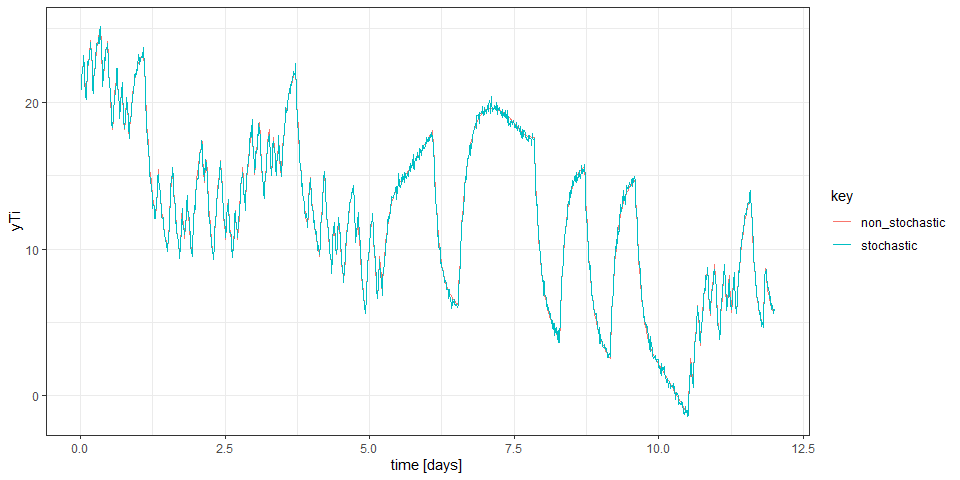
\includegraphics{liu_west_filter_for_a_building_grey_box_model_files/figure-latex/unnamed-chunk-6-1.pdf}

\hypertarget{create-priors}{%
\section{4. Create priors}\label{create-priors}}

As described in section 3.4 Model initialization (Prior generation) in
the paper, we created priors to initialize Liu-West filter.

Define parameter lower and upper bounds that create priors.

\hypertarget{upper-and-lower-bounds-of-states-and-parameter}{%
\subsection{4.1 Upper and lower bounds of states and
parameter}\label{upper-and-lower-bounds-of-states-and-parameter}}

\begin{longtable}[]{@{}lllllll@{}}
\toprule
\begin{minipage}[b]{0.10\columnwidth}\raggedright
\strut
\end{minipage} & \begin{minipage}[b]{0.10\columnwidth}\raggedright
\(T_{\text{i},0}\)\strut
\end{minipage} & \begin{minipage}[b]{0.10\columnwidth}\raggedright
\(T_{\text{e},0}\)\strut
\end{minipage} & \begin{minipage}[b]{0.15\columnwidth}\raggedright
\(C_{\text{i}}\)\strut
\end{minipage} & \begin{minipage}[b]{0.17\columnwidth}\raggedright
\(C_{\text{e}}\)\strut
\end{minipage} & \begin{minipage}[b]{0.10\columnwidth}\raggedright
\(R_{\text{ie}}\)\strut
\end{minipage} & \begin{minipage}[b]{0.10\columnwidth}\raggedright
\(R_{\text{ea}}\)\strut
\end{minipage}\tabularnewline
\midrule
\endhead
\begin{minipage}[t]{0.10\columnwidth}\raggedright
true\strut
\end{minipage} & \begin{minipage}[t]{0.10\columnwidth}\raggedright
21.0\strut
\end{minipage} & \begin{minipage}[t]{0.10\columnwidth}\raggedright
15.0\strut
\end{minipage} & \begin{minipage}[t]{0.15\columnwidth}\raggedright
500000\strut
\end{minipage} & \begin{minipage}[t]{0.17\columnwidth}\raggedright
6000000\strut
\end{minipage} & \begin{minipage}[t]{0.10\columnwidth}\raggedright
1/55\strut
\end{minipage} & \begin{minipage}[t]{0.10\columnwidth}\raggedright
1/55\strut
\end{minipage}\tabularnewline
\begin{minipage}[t]{0.10\columnwidth}\raggedright
min\strut
\end{minipage} & \begin{minipage}[t]{0.10\columnwidth}\raggedright
0\strut
\end{minipage} & \begin{minipage}[t]{0.10\columnwidth}\raggedright
0\strut
\end{minipage} & \begin{minipage}[t]{0.15\columnwidth}\raggedright
100000\strut
\end{minipage} & \begin{minipage}[t]{0.17\columnwidth}\raggedright
1000000\strut
\end{minipage} & \begin{minipage}[t]{0.10\columnwidth}\raggedright
1e-9\strut
\end{minipage} & \begin{minipage}[t]{0.10\columnwidth}\raggedright
1e-9\strut
\end{minipage}\tabularnewline
\begin{minipage}[t]{0.10\columnwidth}\raggedright
max\strut
\end{minipage} & \begin{minipage}[t]{0.10\columnwidth}\raggedright
30.0\strut
\end{minipage} & \begin{minipage}[t]{0.10\columnwidth}\raggedright
30.0\strut
\end{minipage} & \begin{minipage}[t]{0.15\columnwidth}\raggedright
1000000\strut
\end{minipage} & \begin{minipage}[t]{0.17\columnwidth}\raggedright
10000000\strut
\end{minipage} & \begin{minipage}[t]{0.10\columnwidth}\raggedright
0.1\strut
\end{minipage} & \begin{minipage}[t]{0.10\columnwidth}\raggedright
0.1\strut
\end{minipage}\tabularnewline
\bottomrule
\end{longtable}

\begin{Shaded}
\begin{Highlighting}[]
\CommentTok{# define upper and lower bounds of x0 and theta for prior_data.}
\NormalTok{max_x_par=}\KeywordTok{c}\NormalTok{(}\KeywordTok{c}\NormalTok{(}\DecValTok{30}\NormalTok{,}\DecValTok{30}\NormalTok{,}\KeywordTok{c}\NormalTok{(}\DecValTok{1000000}\NormalTok{,}\DecValTok{10000000}\NormalTok{,.}\DecValTok{1}\NormalTok{,}\FloatTok{0.1}\NormalTok{)))}
\NormalTok{min_x_par=}\KeywordTok{c}\NormalTok{(}\DecValTok{10}\NormalTok{,}\DecValTok{0}\NormalTok{,}\DecValTok{100000}\NormalTok{,}\DecValTok{1000000}\NormalTok{,}\FloatTok{1e-9}\NormalTok{,}\FloatTok{1e-9}\NormalTok{)}
\end{Highlighting}
\end{Shaded}

\hypertarget{optimization-to-get-set-of-parameters-eq.-14}{%
\subsection{4.2 Optimization to get set of parameters (Eq.
14)}\label{optimization-to-get-set-of-parameters-eq.-14}}

d

\begin{Shaded}
\begin{Highlighting}[]
\CommentTok{# sometimes optimization fails because cost is NaN. Thus, have this trycatch loop with while so that the optimizer learns again until we get satisfactory number of outcomes.}
\CommentTok{# check optimizer runs. Single run.}
\CommentTok{## library(kfsang) Don't use this library. This package is written by me to have cpp function of nstep function for the speed. Pacakage is not ready-to-publish format.}
\CommentTok{# ss=DEoptim::DEoptim(fn=get_rmse, lower=rep((-0.5+1e-9),length(L_val)),}
\CommentTok{#                      upper=rep(0.5,length(L_val)),control=list(NP=500, itermax=10000,trace=TRUE,reltol=1e-18,steptol=40,parallelType=1,}
\CommentTok{#                                                   parVar=list("discretize_system","nstep_cpp","expm")),}
\CommentTok{#                      dt=dt,u_mat=train_data$u_mat,y_mat=train_data$y_mat,dims=dims,output="cost",normalize=TRUE,L_val=L_val)}

\NormalTok{sol_list=}\KeywordTok{list}\NormalTok{()}
\NormalTok{iii=}\DecValTok{1} 
\ControlFlowTok{while}\NormalTok{(}\KeywordTok{length}\NormalTok{(sol_list)}\OperatorTok{<=}\DecValTok{100}\NormalTok{)\{}
  \KeywordTok{set.seed}\NormalTok{(iii}\OperatorTok{+}\DecValTok{30000}\NormalTok{)}
  \CommentTok{# sometimes optimizer fails since it gives NaN during the nstep-ahead prediction. Thus, we use try-catch.}
\NormalTok{  try_result=}\KeywordTok{tryCatch}\NormalTok{(DEoptim}\OperatorTok{::}\KeywordTok{DEoptim}\NormalTok{(}\DataTypeTok{fn=}\NormalTok{get_rmse, }\DataTypeTok{lower=}\NormalTok{min_x_par}\OperatorTok{/}\NormalTok{max_x_par,}
                     \DataTypeTok{upper=}\NormalTok{max_x_par}\OperatorTok{/}\NormalTok{max_x_par,}
                     \DataTypeTok{control=}\KeywordTok{list}\NormalTok{(}\DataTypeTok{NP=}\DecValTok{100}\NormalTok{, }\DataTypeTok{itermax=}\DecValTok{10000}\NormalTok{,}\DataTypeTok{trace=}\OtherTok{TRUE}\NormalTok{,}\DataTypeTok{reltol=}\FloatTok{1e-16}\NormalTok{,}\DataTypeTok{steptol=}\DecValTok{15}\NormalTok{,}\DataTypeTok{parallelType=}\DecValTok{1}\NormalTok{,}
                                                  \DataTypeTok{parVar=}\KeywordTok{list}\NormalTok{(}\StringTok{"discretize_system"}\NormalTok{,}\StringTok{"nstep"}\NormalTok{,}\StringTok{"expm"}\NormalTok{)),}
                     \DataTypeTok{dt=}\NormalTok{dt,}\DataTypeTok{u_mat=}\NormalTok{prior_data}\OperatorTok{$}\NormalTok{u_mat,}\DataTypeTok{y_mat=}\NormalTok{prior_data}\OperatorTok{$}\NormalTok{y_mat,}\DataTypeTok{dims=}\NormalTok{dims,}\DataTypeTok{output=}\StringTok{"cost"}\NormalTok{,}\DataTypeTok{normalize=}\OtherTok{TRUE}\NormalTok{,}\DataTypeTok{L_val=}\NormalTok{max_x_par)}
\NormalTok{                     ,}
                       \DataTypeTok{error=}\ControlFlowTok{function}\NormalTok{(e)\{}\StringTok{"error"}\NormalTok{\} )}
  
  \ControlFlowTok{if}\NormalTok{((try_result}\OperatorTok{==}\StringTok{"error"}\NormalTok{))\{}
    
\NormalTok{  \}}\ControlFlowTok{else}\NormalTok{\{}
\NormalTok{    sol_list[[(}\KeywordTok{length}\NormalTok{(sol_list)}\OperatorTok{+}\DecValTok{1}\NormalTok{)]]=try_result}
\NormalTok{  \}}
\NormalTok{  iii=iii}\OperatorTok{+}\DecValTok{1}
\NormalTok{\}}
\CommentTok{# store solution.}
\KeywordTok{write_rds}\NormalTok{(sol_list,}\KeywordTok{paste0}\NormalTok{(}\StringTok{"data/sol_list.rds"}\NormalTok{))}
\end{Highlighting}
\end{Shaded}

\hypertarget{visualize-obtained-set-of-parameters}{%
\subsection{4.3 Visualize obtained set of
parameters}\label{visualize-obtained-set-of-parameters}}

To run Liu-West filter on the \texttt{filter\_data}, we need both prior
for initial states and parameters. In 3.3.2, initial states and
parameters of \texttt{prior\_data} are obtained from optimizer. The
initial states of \texttt{filter\_data} is actually the last states of
\texttt{prior\_data}. Therefore, we do \texttt{n-step} ahead prediction
on \texttt{prior\_data} with set of parameters from the obtimizer to
have initial states of \texttt{filter\_data}.

\begin{Shaded}
\begin{Highlighting}[]
\CommentTok{# load results}
\NormalTok{sol_list=readr}\OperatorTok{::}\KeywordTok{read_rds}\NormalTok{(}\KeywordTok{paste0}\NormalTok{(}\StringTok{"data/sol_list.rds"}\NormalTok{))}


\CommentTok{# sol_list contains intial states and parameters of prior_data.}
\CommentTok{# we will have initial state and parameters for filter_data in sol_list_temp}
\NormalTok{sol_list_temp=}\KeywordTok{list}\NormalTok{()}

\ControlFlowTok{for}\NormalTok{ (i }\ControlFlowTok{in} \DecValTok{1}\OperatorTok{:}\KeywordTok{length}\NormalTok{(sol_list))\{}
\NormalTok{  sol_list_temp[[i]]=(sol_list[[i]]}\OperatorTok{$}\NormalTok{optim}\OperatorTok{$}\NormalTok{bestmem)}\OperatorTok{*}\NormalTok{max_x_par }\CommentTok{#extract optimizer solution and unnormalize it.}
  \CommentTok{# store n-step ahead prediction result}
  \CommentTok{# 1:index_split: prior data, index_split+1:index_split*2: filter_data}
\NormalTok{  tempp=}\KeywordTok{get_rmse}\NormalTok{(}\DataTypeTok{par=}\NormalTok{sol_list_temp[[i]],}\DataTypeTok{dt=}\NormalTok{dt,}
                 \DataTypeTok{u_mat=}\NormalTok{all_data}\OperatorTok{$}\NormalTok{u_mat[,}\DecValTok{1}\OperatorTok{:}\NormalTok{(index_split}\OperatorTok{+}\DecValTok{1}\NormalTok{)],}
                 \DataTypeTok{y_mat=}\NormalTok{all_data}\OperatorTok{$}\NormalTok{y_mat[}\DecValTok{1}\OperatorTok{:}\NormalTok{(index_split}\OperatorTok{+}\DecValTok{1}\NormalTok{)],}
                 \DataTypeTok{dims=}\NormalTok{dims,}\DataTypeTok{output=}\StringTok{"data"}\NormalTok{,}\DataTypeTok{normalize=}\OtherTok{FALSE}\NormalTok{)}
  \CommentTok{# put indepx_split+1 states into initial states into sol_list. }
\NormalTok{  sol_list_temp[[i]][}\DecValTok{1}\OperatorTok{:}\DecValTok{2}\NormalTok{]=tempp}\OperatorTok{$}\NormalTok{x_pred[,index_split}\OperatorTok{+}\DecValTok{1}\NormalTok{]}
\NormalTok{\}}


\CommentTok{# sol_list_temp to dataframe}
\NormalTok{all_df=}\KeywordTok{do.call}\NormalTok{(rbind,sol_list_temp)}\OperatorTok\KeywordTok{as_tibble}\NormalTok{()}

\NormalTok{state_names<-}\KeywordTok{c}\NormalTok{(}\StringTok{"Ti0"}\NormalTok{,}\StringTok{"Te0"}\NormalTok{)}
\NormalTok{par_name<-}\KeywordTok{c}\NormalTok{(}\StringTok{"Ci"}\NormalTok{,}\StringTok{"Ce"}\NormalTok{,}\StringTok{"Rie"}\NormalTok{,}\StringTok{"Rea"}\NormalTok{)}
\CommentTok{# split data_frame into state/parameter}
\NormalTok{par_df=all_df[,}\OperatorTok{-}\KeywordTok{c}\NormalTok{(}\DecValTok{1}\OperatorTok{:}\DecValTok{2}\NormalTok{)]}\OperatorTok\KeywordTok{set_names}\NormalTok{(par_name)}
\NormalTok{state_df=all_df[,}\DecValTok{1}\OperatorTok{:}\DecValTok{2}\NormalTok{]}\OperatorTok\KeywordTok{set_names}\NormalTok{(state_names)}
\CommentTok{# data_frame for visualization}
\NormalTok{par_df_plot<-par_df}\OperatorTok\KeywordTok{mutate}\NormalTok{(}\DataTypeTok{type=}\StringTok{"data"}\NormalTok{)}
\CommentTok{# add true parameter into data frame for visualization}
\NormalTok{par_true_df=par_true[}\DecValTok{1}\OperatorTok{:}\KeywordTok{length}\NormalTok{(par_name)]}

\KeywordTok{names}\NormalTok{(par_true_df)<-par_name}
\NormalTok{par_true_df=par_true_df}\OperatorTok\KeywordTok{as.list}\NormalTok{()}\OperatorTok\KeywordTok{as_tibble}\NormalTok{()}\OperatorTok\KeywordTok{mutate}\NormalTok{(}\DataTypeTok{type=}\StringTok{"true"}\NormalTok{)}

\NormalTok{par_df_plot=}\KeywordTok{bind_rows}\NormalTok{(par_df_plot,par_true_df)}


\KeywordTok{library}\NormalTok{(ggforce)}

\NormalTok{cols <-}\StringTok{ }\KeywordTok{c}\NormalTok{(}\StringTok{"data"}\NormalTok{ =}\StringTok{ "black"}\NormalTok{, }\StringTok{"true"}\NormalTok{ =}\StringTok{ "red"}\NormalTok{)}
\CommentTok{# Ti,0  Te,0,   Ce, Ci  Rea Rie }
\KeywordTok{ggplot}\NormalTok{(par_df_plot, }\KeywordTok{aes}\NormalTok{(}\DataTypeTok{x =}\NormalTok{ .panel_x, }\DataTypeTok{y =}\NormalTok{ .panel_y,}\DataTypeTok{color=}\NormalTok{type,}\DataTypeTok{fill=}\NormalTok{type)) }\OperatorTok{+}\StringTok{ }
\StringTok{  }\KeywordTok{geom_point}\NormalTok{(}\DataTypeTok{alpha =} \FloatTok{1.0}\NormalTok{, }\DataTypeTok{shape =} \DecValTok{16}\NormalTok{, }\DataTypeTok{size =} \FloatTok{2.0}\NormalTok{) }\OperatorTok{+}\StringTok{ }
\StringTok{  }\KeywordTok{facet_matrix}\NormalTok{(}\KeywordTok{vars}\NormalTok{(}\OperatorTok{-}\NormalTok{type),}\DataTypeTok{layer.lower =}\NormalTok{ T,}\DataTypeTok{layer.diag =}\NormalTok{ T, }\DataTypeTok{layer.upper =}\NormalTok{ F)}\OperatorTok{+}
\StringTok{  }\KeywordTok{scale_colour_manual}\NormalTok{(}\DataTypeTok{values =}\NormalTok{ cols)}\OperatorTok{+}\KeywordTok{theme_bw}\NormalTok{()}\OperatorTok{+}\KeywordTok{theme}\NormalTok{(}\DataTypeTok{axis.text.x =} \KeywordTok{element_text}\NormalTok{(}\DataTypeTok{angle =} \DecValTok{90}\NormalTok{))}
\end{Highlighting}
\end{Shaded}

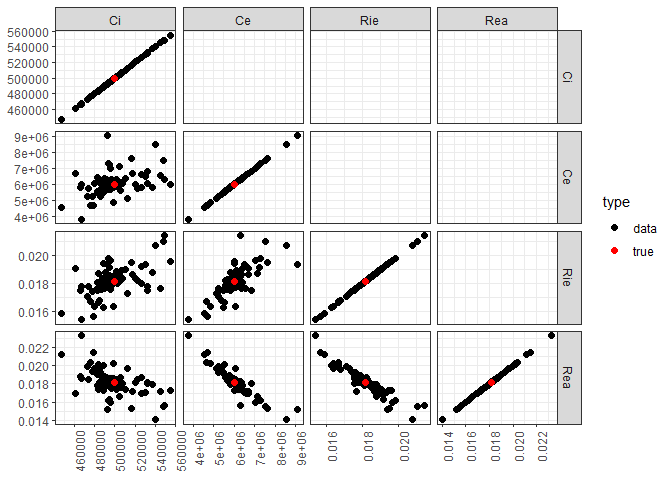
\includegraphics{liu_west_filter_for_a_building_grey_box_model_files/figure-latex/unnamed-chunk-9-1.pdf}

\hypertarget{kernel-density-approximation-of-set-of-pameters}{%
\subsection{4.4 Kernel density approximation of set of
pameters}\label{kernel-density-approximation-of-set-of-pameters}}

\begin{Shaded}
\begin{Highlighting}[]
\KeywordTok{suppressPackageStartupMessages}\NormalTok{(}\KeywordTok{library}\NormalTok{(kdevine))}
\CommentTok{# multivariate kernel density approximation}
\NormalTok{kde_par <-}\StringTok{ }\NormalTok{kdevine}\OperatorTok{::}\KeywordTok{kdevine}\NormalTok{(}\KeywordTok{as.matrix}\NormalTok{(par_df)) }\CommentTok{#kernel model K(x)}
\NormalTok{kde_state <-}\StringTok{ }\NormalTok{kdevine}\OperatorTok{::}\KeywordTok{kdevine}\NormalTok{(}\KeywordTok{as.matrix}\NormalTok{(state_df)) }\CommentTok{#kernel model K(theta)}

\CommentTok{# Generate }
\NormalTok{set.seed=}\DecValTok{104}
\NormalTok{NP=}\DecValTok{10000}
\NormalTok{prior_par=Rfast}\OperatorTok{::}\KeywordTok{transpose}\NormalTok{(}\KeywordTok{abs}\NormalTok{(kdevine}\OperatorTok{::}\KeywordTok{rkdevine}\NormalTok{(NP, kde_par)))}
\NormalTok{prior_state=Rfast}\OperatorTok{::}\KeywordTok{transpose}\NormalTok{(kdevine}\OperatorTok{::}\KeywordTok{rkdevine}\NormalTok{(NP, kde_state))}


\KeywordTok{write_rds}\NormalTok{(kde_par,}\KeywordTok{paste0}\NormalTok{(}\StringTok{"data/kde_par.rds"}\NormalTok{))}
\KeywordTok{write_rds}\NormalTok{(kde_state,}\KeywordTok{paste0}\NormalTok{(}\StringTok{"data/kde_state.rds"}\NormalTok{))}
\KeywordTok{write_rds}\NormalTok{(prior_par,}\KeywordTok{paste0}\NormalTok{(}\StringTok{"data/prior_par.rds"}\NormalTok{))}
\KeywordTok{write_rds}\NormalTok{(prior_state,}\KeywordTok{paste0}\NormalTok{(}\StringTok{"data/prior_state.rds"}\NormalTok{))}
\end{Highlighting}
\end{Shaded}

\hypertarget{kernel-density-approximation-of-set-of-pameters-1}{%
\subsection{4. Kernel density approximation of set of
pameters}\label{kernel-density-approximation-of-set-of-pameters-1}}

\begin{Shaded}
\begin{Highlighting}[]
\CommentTok{# load generated prior data from the kernel density approximation}
\NormalTok{prior_par=readr}\OperatorTok{::}\KeywordTok{read_rds}\NormalTok{(}\KeywordTok{paste0}\NormalTok{(}\StringTok{"data/prior_par.rds"}\NormalTok{))}
\NormalTok{prior_state=readr}\OperatorTok{::}\KeywordTok{read_rds}\NormalTok{(}\KeywordTok{paste0}\NormalTok{(}\StringTok{"data/prior_state.rds"}\NormalTok{))}
\NormalTok{NP=}\KeywordTok{dim}\NormalTok{(prior_par)[}\DecValTok{2}\NormalTok{]}


\CommentTok{# permutate gerenated prior to have uniform weight in a wide range}
\NormalTok{min_val=}\KeywordTok{floor}\NormalTok{(}\KeywordTok{min}\NormalTok{(prior_par[}\DecValTok{1}\NormalTok{,])) }\CommentTok{# minimum bounds of single parameter elemenet  }
\NormalTok{max_val=}\KeywordTok{ceiling}\NormalTok{(}\KeywordTok{max}\NormalTok{(prior_par[}\DecValTok{1}\NormalTok{,])) }\CommentTok{# maximum bounds of single parameter elemenet }
\NormalTok{min_max_grid=}\KeywordTok{seq}\NormalTok{(min_val,max_val,}\DataTypeTok{length.out=}\NormalTok{NP) }\CommentTok{# parameter grids based on the min/max range.}
\NormalTok{permutation_grid=}\KeywordTok{sapply}\NormalTok{(}\DecValTok{1}\OperatorTok{:}\NormalTok{NP,}\ControlFlowTok{function}\NormalTok{(x) }\KeywordTok{which.min}\NormalTok{(}\KeywordTok{abs}\NormalTok{(prior_par[}\DecValTok{1}\NormalTok{,]}\OperatorTok{-}\NormalTok{min_max_grid[x])))}
\NormalTok{prior_par=prior_par[,permutation_grid]}
\NormalTok{prior_state=prior_state[,permutation_grid]}

\CommentTok{# create data_frame for visualization}
\NormalTok{prior_par_df=prior_par}\OperatorTok\NormalTok{Rfast}\OperatorTok{::}\KeywordTok{transpose}\NormalTok{()}\OperatorTok
\StringTok{  }\KeywordTok{as.data.frame}\NormalTok{()}\OperatorTok\KeywordTok{as_tibble}\NormalTok{()}\OperatorTok\KeywordTok{set_names}\NormalTok{(par_name[}\DecValTok{1}\OperatorTok{:}\NormalTok{(}\KeywordTok{dim}\NormalTok{(prior_par)[}\DecValTok{1}\NormalTok{])])}

\NormalTok{par_df_plot2=}\KeywordTok{bind_rows}\NormalTok{(prior_par_df}\OperatorTok\KeywordTok{mutate}\NormalTok{(}\DataTypeTok{type=}\StringTok{"prior"}\NormalTok{),par_df}\OperatorTok\KeywordTok{mutate}\NormalTok{(}\DataTypeTok{type=}\StringTok{"optimizer"}\NormalTok{))}

\NormalTok{cols2 <-}\StringTok{ }\KeywordTok{c}\NormalTok{(}\StringTok{"optimizer"}\NormalTok{ =}\StringTok{ "red"}\NormalTok{, }\StringTok{"prior"}\NormalTok{ =}\StringTok{ "grey75"}\NormalTok{)}
\KeywordTok{ggplot}\NormalTok{(par_df_plot2, }\KeywordTok{aes}\NormalTok{(}\DataTypeTok{x =}\NormalTok{ .panel_x, }\DataTypeTok{y =}\NormalTok{ .panel_y,}\DataTypeTok{color=}\NormalTok{type,}\DataTypeTok{fill=}\NormalTok{type)) }\OperatorTok{+}\StringTok{ }
\StringTok{  }\KeywordTok{geom_point}\NormalTok{(}\DataTypeTok{alpha =} \FloatTok{0.3}\NormalTok{, }\DataTypeTok{shape =} \DecValTok{16}\NormalTok{, }\DataTypeTok{size =} \FloatTok{1.5}\NormalTok{) }\OperatorTok{+}\StringTok{ }
\StringTok{  }\KeywordTok{facet_matrix}\NormalTok{(}\KeywordTok{vars}\NormalTok{(}\OperatorTok{-}\NormalTok{type),}\DataTypeTok{layer.lower =}\NormalTok{ T,}\DataTypeTok{layer.diag =}\NormalTok{ T, }\DataTypeTok{layer.upper =}\NormalTok{ F)}\OperatorTok{+}
\StringTok{  }\KeywordTok{scale_colour_manual}\NormalTok{(}\DataTypeTok{values =}\NormalTok{ cols2)}\OperatorTok{+}
\StringTok{  }\KeywordTok{scale_fill_manual}\NormalTok{(}\DataTypeTok{values =}\NormalTok{ cols2)}\OperatorTok{+}
\StringTok{  }\KeywordTok{theme_bw}\NormalTok{()}\OperatorTok{+}\KeywordTok{theme}\NormalTok{(}\DataTypeTok{axis.text.x =} \KeywordTok{element_text}\NormalTok{(}\DataTypeTok{angle =} \DecValTok{90}\NormalTok{))}
\end{Highlighting}
\end{Shaded}

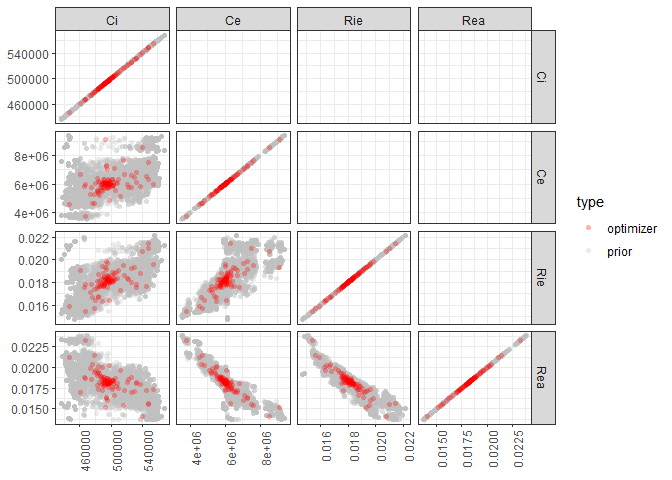
\includegraphics{liu_west_filter_for_a_building_grey_box_model_files/figure-latex/unnamed-chunk-11-1.pdf}

\hypertarget{liu-west-filter}{%
\section{5. Liu-West filter}\label{liu-west-filter}}

Since we have priors, we can run Liu-West filter. For complete algorithm
of the filter, refer Table 2 in the paper.

\begin{Shaded}
\begin{Highlighting}[]
\CommentTok{# L_values of parameter to normalize parameters}
\NormalTok{L_val_par=}\KeywordTok{apply}\NormalTok{(prior_par,}\DataTypeTok{MARGIN=}\KeywordTok{c}\NormalTok{(}\DecValTok{1}\NormalTok{),max) }
\NormalTok{prior_par_n=(prior_par)}\OperatorTok{/}\NormalTok{L_val_par}\FloatTok{-0.5} \CommentTok{#normalized parameter }
\NormalTok{num_state=}\KeywordTok{dim}\NormalTok{(prior_state)[}\DecValTok{1}\NormalTok{] }\CommentTok{# number of state}


\CommentTok{# define L_values of noise parameter (sigma_x_i,sigma_x_e)}
\NormalTok{L_val_sd=}\KeywordTok{rep}\NormalTok{(.}\DecValTok{1}\OperatorTok{/}\KeywordTok{sqrt}\NormalTok{(dt),num_state) }
\NormalTok{L_val=}\KeywordTok{c}\NormalTok{(L_val_par,L_val_sd) }\CommentTok{#L_val for parameter +noise parameter}

\CommentTok{# normalized priors for noise parameter by using Ratin-Hyper cube sampling}
\KeywordTok{set.seed}\NormalTok{(}\DecValTok{1234}\NormalTok{)}
\NormalTok{prior_sd_n=(Rfast}\OperatorTok{::}\KeywordTok{transpose}\NormalTok{(lhs}\OperatorTok{::}\KeywordTok{randomLHS}\NormalTok{(NP,}\KeywordTok{length}\NormalTok{(L_val)}\OperatorTok{-}\NormalTok{(}\KeywordTok{dim}\NormalTok{(prior_par_n)[}\DecValTok{1}\NormalTok{] ))))}\OperatorTok{-}\FloatTok{0.5}

\CommentTok{# all normalized parameters.}
\NormalTok{prior_all_n=}\KeywordTok{rbind}\NormalTok{(prior_par_n,prior_sd_n)}
\NormalTok{num_par=}\KeywordTok{dim}\NormalTok{(prior_all_n)[}\DecValTok{1}\NormalTok{]}

\CommentTok{# initial x0}
\NormalTok{x=prior_state }\CommentTok{#x0}
\NormalTok{pii=w=}\KeywordTok{rep}\NormalTok{(}\DecValTok{1}\OperatorTok{/}\NormalTok{NP,NP) }\CommentTok{#initilal weight}

\CommentTok{# inputs for the model}
\NormalTok{inputs=}\KeywordTok{list}\NormalTok{()}
\NormalTok{inputs}\OperatorTok{$}\NormalTok{L_val=L_val }\CommentTok{#L_val for normalization/unnormalization.}
\NormalTok{inputs}\OperatorTok{$}\NormalTok{dt=dt }\CommentTok{#time interval}

\NormalTok{inputs}\OperatorTok{$}\NormalTok{y_mat=filter_data}\OperatorTok{$}\NormalTok{y_mat }\CommentTok{# y_data}
\NormalTok{inputs}\OperatorTok{$}\NormalTok{u_mat=filter_data}\OperatorTok{$}\NormalTok{u_mat }\CommentTok{# input u_data}

\CommentTok{# parameter names}
\NormalTok{par_names=}\KeywordTok{c}\NormalTok{(}\StringTok{"Ci"}\NormalTok{,}\StringTok{"Ce"}\NormalTok{,}\StringTok{"Rie"}\NormalTok{,}\StringTok{"Rea"}\NormalTok{,}\StringTok{"sdte"}\NormalTok{,}\StringTok{"sdti"}\NormalTok{)}
\NormalTok{inputs}\OperatorTok{$}\NormalTok{par_names=par_names}

\CommentTok{# initial parameter prior particles}
\NormalTok{theta=prior_all_n}
\NormalTok{delta=}\FloatTok{0.9} \CommentTok{# Filter tuning parameter }
\NormalTok{seed_num=}\DecValTok{13244} \CommentTok{#seed number}
\end{Highlighting}
\end{Shaded}

\begin{Shaded}
\begin{Highlighting}[]
\CommentTok{# seed=seed_num}
\CommentTok{#res=lw_ss_filter(inputs=inputs,NP=NP,pii=pii,x=x,theta=theta,wt=wt,seed=seed_num,training=TRUE)}
\NormalTok{res=}\KeywordTok{lw_ss_filter}\NormalTok{(}\DataTypeTok{inputs=}\NormalTok{inputs,}\DataTypeTok{NP=}\NormalTok{NP,}\DataTypeTok{pii=}\NormalTok{pii,}\DataTypeTok{x=}\NormalTok{x,}\DataTypeTok{theta=}\NormalTok{theta,}\DataTypeTok{delta=}\NormalTok{delta,}\DataTypeTok{seed=}\NormalTok{seed_num,}\DataTypeTok{training=}\OtherTok{TRUE}\NormalTok{)}



\ControlFlowTok{for}\NormalTok{(i }\ControlFlowTok{in} \DecValTok{1}\OperatorTok{:}\KeywordTok{dim}\NormalTok{(res}\OperatorTok{$}\NormalTok{r_thetas)[}\DecValTok{1}\NormalTok{])\{}
  \KeywordTok{write_rds}\NormalTok{(res}\OperatorTok{$}\NormalTok{r_thetas[i,,],}\KeywordTok{paste0}\NormalTok{(}\StringTok{"data/res_thetas_"}\NormalTok{,i,}\StringTok{".rds"}\NormalTok{))}
\NormalTok{\}}
\ControlFlowTok{for}\NormalTok{(i }\ControlFlowTok{in} \DecValTok{1}\OperatorTok{:}\KeywordTok{dim}\NormalTok{(res}\OperatorTok{$}\NormalTok{xs)[}\DecValTok{1}\NormalTok{])\{}
  \KeywordTok{write_rds}\NormalTok{(res}\OperatorTok{$}\NormalTok{xs[i,,],}\KeywordTok{paste0}\NormalTok{(}\StringTok{"data/res_xs_"}\NormalTok{,i,}\StringTok{".rds"}\NormalTok{))}
\NormalTok{\}}

\NormalTok{res}\OperatorTok{$}\NormalTok{thetas<-}\OtherTok{NULL}
\NormalTok{res}\OperatorTok{$}\NormalTok{r_thetas<-}\OtherTok{NULL}
\NormalTok{res}\OperatorTok{$}\NormalTok{xs<-}\OtherTok{NULL}
\KeywordTok{write_rds}\NormalTok{(res,}\StringTok{"data/res.rds"}\NormalTok{)}
\end{Highlighting}
\end{Shaded}

\begin{Shaded}
\begin{Highlighting}[]
\NormalTok{res=}\KeywordTok{read_rds}\NormalTok{(}\StringTok{"data/res.rds"}\NormalTok{)}

\NormalTok{res}\OperatorTok{$}\NormalTok{r_thetas=}\KeywordTok{array}\NormalTok{(}\DataTypeTok{data=}\DecValTok{0}\NormalTok{,}\DataTypeTok{dim=}\KeywordTok{c}\NormalTok{(}\KeywordTok{length}\NormalTok{(par_names),NP,}\KeywordTok{dim}\NormalTok{(filter_data}\OperatorTok{$}\NormalTok{u_mat)[}\DecValTok{2}\NormalTok{]))}
\NormalTok{res}\OperatorTok{$}\NormalTok{xs=}\KeywordTok{array}\NormalTok{(}\DataTypeTok{data=}\DecValTok{0}\NormalTok{,}\DataTypeTok{dim=}\KeywordTok{c}\NormalTok{(}\KeywordTok{length}\NormalTok{(state_names),NP,}\KeywordTok{dim}\NormalTok{(filter_data}\OperatorTok{$}\NormalTok{u_mat)[}\DecValTok{2}\NormalTok{]))}
\ControlFlowTok{for}\NormalTok{ (i }\ControlFlowTok{in} \DecValTok{1}\OperatorTok{:}\KeywordTok{length}\NormalTok{(par_names))\{}
\NormalTok{  res}\OperatorTok{$}\NormalTok{r_thetas[i,,]=}\KeywordTok{read_rds}\NormalTok{(}\KeywordTok{paste0}\NormalTok{(}\StringTok{"data/res_thetas_"}\NormalTok{,i,}\StringTok{".rds"}\NormalTok{))}
\NormalTok{\}}

\ControlFlowTok{for}\NormalTok{ (i }\ControlFlowTok{in} \DecValTok{1}\OperatorTok{:}\KeywordTok{length}\NormalTok{(state_names))\{}
\NormalTok{  res}\OperatorTok{$}\NormalTok{xs[i,,]=}\KeywordTok{read_rds}\NormalTok{(}\KeywordTok{paste0}\NormalTok{(}\StringTok{"data/res_xs_"}\NormalTok{,i,}\StringTok{".rds"}\NormalTok{))}
\NormalTok{\}}
\CommentTok{# res$xs[1,,]%>%colMeans%>%plot(type='l')}
\CommentTok{# filter_data$y_mat%>%points(type='l',col="red")}
\CommentTok{# res$xs[2,,]%>%colMeans%>%plot()}



\CommentTok{#theta_quantile=res$thetas%>%apply(MARGIN=c(2,3),function (x) quantile(x,c(0.025,0.5,0.975)))}
\NormalTok{rtheta_quantile=res}\OperatorTok{$}\NormalTok{r_thetas}\OperatorTok\KeywordTok{apply}\NormalTok{(}\DataTypeTok{MARGIN=}\KeywordTok{c}\NormalTok{(}\DecValTok{1}\NormalTok{,}\DecValTok{3}\NormalTok{),}\ControlFlowTok{function}\NormalTok{ (x) }\KeywordTok{quantile}\NormalTok{(x,}\KeywordTok{c}\NormalTok{(}\FloatTok{0.025}\NormalTok{,}\FloatTok{0.5}\NormalTok{,}\FloatTok{0.975}\NormalTok{)))}
\CommentTok{#par_names=names(par_recover_lw(1,res$lw_mean,res$lw_sd))}
\NormalTok{par_name=}\KeywordTok{c}\NormalTok{(}\StringTok{"Ci"}\NormalTok{,}\StringTok{"Ce"}\NormalTok{,}\StringTok{"Rie"}\NormalTok{,}\StringTok{"Rea"}\NormalTok{)}

\ControlFlowTok{for}\NormalTok{ (i }\ControlFlowTok{in} \DecValTok{1}\OperatorTok{:}\DecValTok{4}\NormalTok{)\{}
\NormalTok{  theta_idx=i}
  \KeywordTok{plot}\NormalTok{(rtheta_quantile[}\DecValTok{2}\NormalTok{,theta_idx,],}\DataTypeTok{col=}\StringTok{"black"}\NormalTok{,}\DataTypeTok{type=}\StringTok{"l"}\NormalTok{,}\DataTypeTok{ylim=}\KeywordTok{c}\NormalTok{(}\KeywordTok{min}\NormalTok{(rtheta_quantile[,theta_idx,],par_true[theta_idx]),}\KeywordTok{max}\NormalTok{(rtheta_quantile[,theta_idx,],par_true[theta_idx])),}
       \DataTypeTok{ylab=}\KeywordTok{paste0}\NormalTok{(par_name[theta_idx]))}
  \KeywordTok{lines}\NormalTok{(rtheta_quantile[}\DecValTok{1}\NormalTok{,theta_idx,],}\DataTypeTok{col=}\StringTok{"blue"}\NormalTok{)}
  \KeywordTok{lines}\NormalTok{(rtheta_quantile[}\DecValTok{3}\NormalTok{,theta_idx,],}\DataTypeTok{col=}\StringTok{"blue"}\NormalTok{)}
  \KeywordTok{abline}\NormalTok{(}\DataTypeTok{h=}\NormalTok{par_true[theta_idx],}\DataTypeTok{col=}\StringTok{"red"}\NormalTok{)}
\NormalTok{\}}
\end{Highlighting}
\end{Shaded}

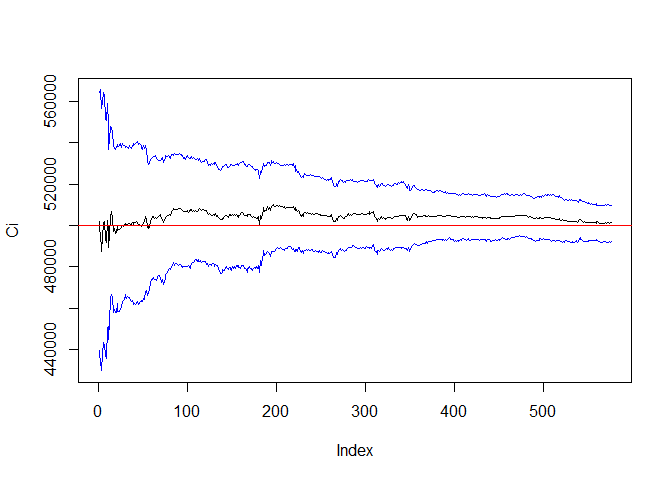
\includegraphics{liu_west_filter_for_a_building_grey_box_model_files/figure-latex/unnamed-chunk-14-1.pdf}
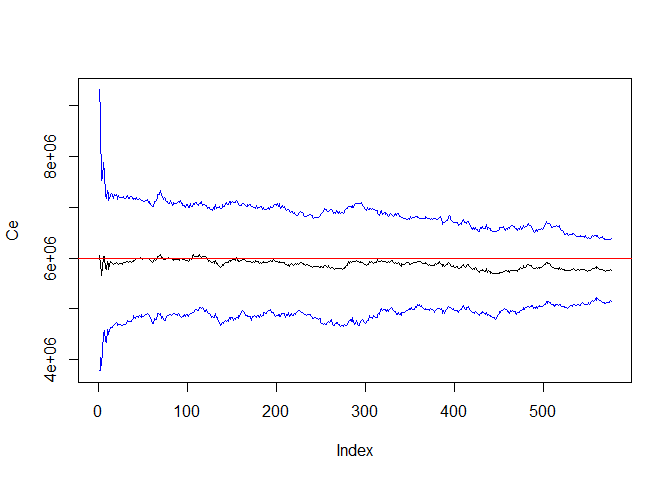
\includegraphics{liu_west_filter_for_a_building_grey_box_model_files/figure-latex/unnamed-chunk-14-2.pdf}
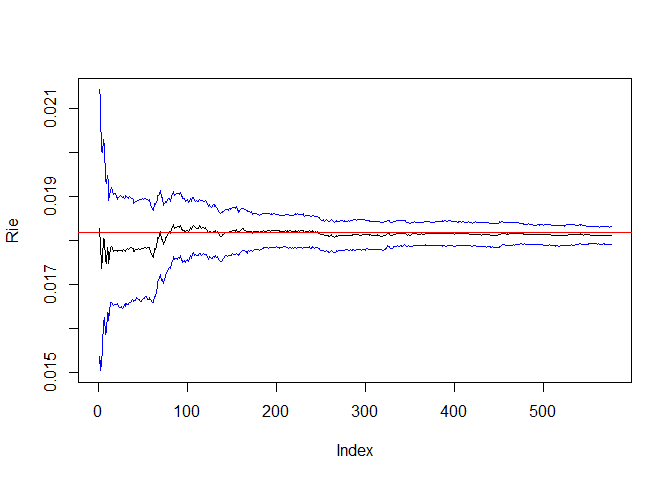
\includegraphics{liu_west_filter_for_a_building_grey_box_model_files/figure-latex/unnamed-chunk-14-3.pdf}
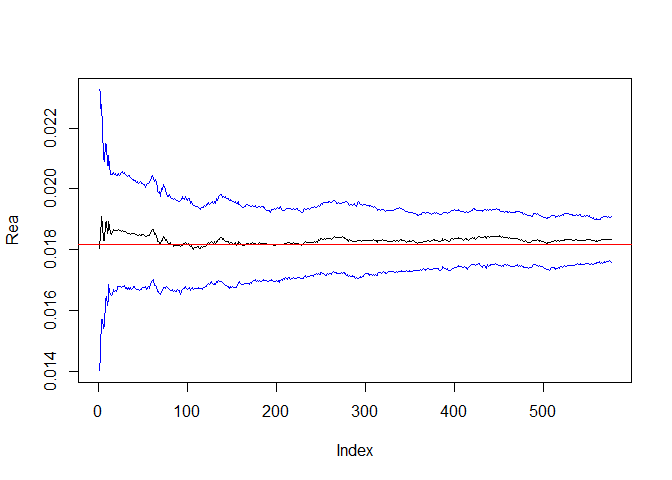
\includegraphics{liu_west_filter_for_a_building_grey_box_model_files/figure-latex/unnamed-chunk-14-4.pdf}

\end{document}
